\newpage
\thispagestyle{empty}
\section{Einleitung Neuronale Netze}\label{sec:einleitung_nn}   
NN (wofür, Einsatzgebiete, Grobes Prinzip). EINFÜGEN

\vspace{1cm}
\begin{tcolorbox}[title={Inhalt}]
Die Einleitung umfasst folgende Elemente\footnote{Vgl. u.a. \cite{BBoJ}, S. 5-6}:
\begin{itemize}
\item Wofür benötigt man Neuronale Netze
\item Einsatzgebiete
\item Grobes Prinzip
  \begin{quotation}
    Eine Einleitung muss auch durch die Arbeit führen. Sie muss dem Leser helfen, sich in der Arbeit und ihrer Struktur zu Recht zu finden. Für jedes Kapitel sollte eine ganz kurze Inhaltsangabe gemacht werden und ggf. motiviert werden, warum es geschrieben wurde. Oft denkt sich ein Autor etwas bei der Struktur seiner Arbeit, auch solche Beweggründe sind dem Leser zu erklären\footnote{\cite{BBoJ}, S. 6}:. 
  \end{quotation}
\end{itemize}
\end{tcolorbox}

\subsection{Wofür benötigt man Neuronale Netze}\label{subsec:einleitung_nn:wofuer_nn} 

\subsection{Einsatzgebiete}\label{subsec:einleitung_nn:einsatzgebiete}

\subsection{Grobes Prinzip}\label{subsec:einleitung_nn_grobes:prinzip}


%Neuronen 
\newpage  
\section{Neuronen}\label{sec:neuronen}
  \begin{tcolorbox}[title={Inhalt}]
\begin{itemize} 
    \item Was sind Neuronen
    \item Arten von Neuronen
    \item Funktionsweise
    \item Aktivierungsfunktion
    \item Schichtenmodell
\end{itemize} 
\end{tcolorbox}
\subsection{Was sind Neuronen?}\label{sec:neuronen:was_sind_neuronen}  
Das menschliche Nervensystem besteht aus Neuronen, welche mit Axonen oder Dendriten verknüpft sind. Diese Verbindungen werden auch Synapsen genannt. Die variable Stärke der Synapsen
ermöglichen das Lernen. Dieser biologische Mechanismus wird durch neurale Netze simuliert.\\

\begin{figure}[H]
\begin{subfigure}{0.6\textwidth}
    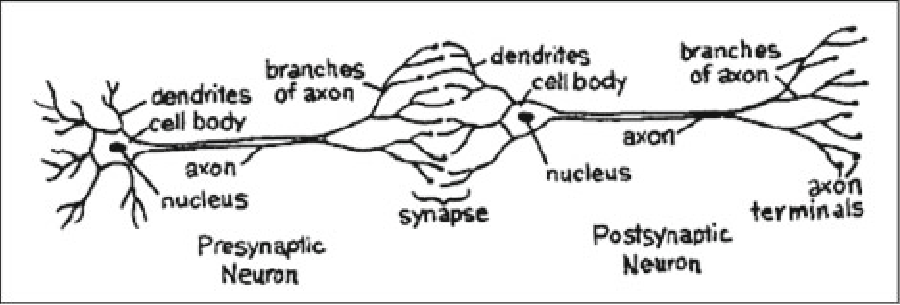
\includegraphics[width=\textwidth]{Sources/01-01_synapse.png}
    \label{Synapse}
    \caption{Synapse}
\end{subfigure}
\begin{subfigure}{0.25\textwidth}
    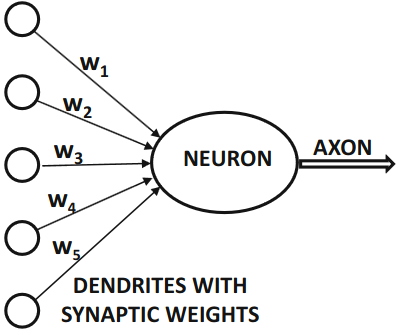
\includegraphics[width=\textwidth]{Sources/01-02_neuron.png}
    \label{Neuron}
    \caption{Neuron}
\end{subfigure}
\caption{Neural Networks and Deep Learning A Textbook, Charu C. Aggarwal
}
\end{figure}

Eines neuronales Netz besteht aus mindestens einem Neuron. Neuronen sind essentielle Bestandteile von neuralen Netzen. Sie nehmen Eingabedaten entgegen und wandeln diese 
in Ausgabedaten um. Neben den Eingabedaten werden auch Weight-Parameter übergeben, welche die zu berechnenden Werte beinflussen. Das eigenliche \enquote{Lernen} erfolgt durch diesen 
Einfluss.
\subsection{Arten von Neuronen}\label{subsec:neuronen:arten_von_neuronen}
  TEXT FOLGT... 
\newpage
\subsection{Funktionsweise}\label{subsec:neuronen:funktionsweise}
  %\input{}
  TEXT FOLGT... 
 

\newpage
\subsubsection{Aktivierungsfunktion}\label{subsec:neuronen:aktivierungsfunktion}
  Aktivierungsfunktionen ermöglichen den Neuronen nicht-lineare Outputs zu produzieren. Außerdem wird durch diese Funktionen entschieden, 
welche Neuronen aktiviert werden und wie die Inputs gewichtet werden. Zur Notation von Aktivierungsfunktion nutzen wir $\Phi$.
$$\hat{y} = \Phi(\overline{W} \cdot \overline{X})$$
\paragraph{Lineare Aktivierung}
Die simpelste Aktivierungsfunktion $\Phi(\cdot)$ ist die lineare Aktivierung. Sie bietet keine nicht linearität. Sie wird oft in Output Nodes
verwendet, wenn das Ziel ein reeler Wert ist.
$$\Phi(v) = v$$
\paragraph{Nicht lineare Aktivierung}
In den frühen Tagen der Entwicklung von neuralen Netzen wurden sign, sigmoid und hyperbolic tangent Funktionen genutzt.
\subparagraph{Sign Aktivierung}
Die sign Funktion generiert nur binäre \{-1,+1\} Ausgaben. Aufgrund der Nichtstätigkeit der Funktion, können beim Trainieren keine Loss-Funktionen verwendet werden.
$$\Phi(v) = \text{sign}(v)$$
\subparagraph{Sigmoid Aktivierung}
Die Sigmoid Funktion generiert Werte zwischen 0 und 1. Sie eignet sich deshalb für Rechnungen die als Wahrscheinlichkeiten interpetiert werden sollen.
$$\Phi(v) = \frac{1}{1 + e^{-v}}$$
\subparagraph{Tanh Aktivierung}
Der Graph der Tanh Funktion hat eine ähneliche Form wie die der Sigmoid Funktion. Sie unterscheidet sich jedoch in der Skalierung, denn ihre Wertebereich liegt zwischen -1 und 1.
$$\Phi(v) = \frac{e^{2v} - 1}{e^{2v} + 1}$$
Die Tanh Funktion lässt sich auch durch die Sigmoid Funktion darstellen.
$$\text{tanh}(v) = 2 \cdot \text{sigmoid}(2v) - 1$$
Wenn die Ausgabe der Berechnung postitiv sowie negativ sein kann, ist die tanh Funktion der sigmoid Funktion vorzuziehen. Außerdem ist es einfacher zu trainieren, weil die Funktion Mittelwertzentriert
und der Gradient größer ist.

\paragraph{Piecewise lineare Aktivierung}
Historisch wurden die Sigmoid und Tanh Funktion zur Einführung von Nichtliniearität genutzt. Heutzutage sind piecewise linear activation Funktionen (Stückweise Linear) beliebter, weil diese das Trainieren 
von mehrschichtigen neuronalen Netzen einfacher machen.
\subparagraph{ReLU}
TODO\\
$$\Phi(v) = \text{max}\{v,0\}$$
\subparagraph{hard tanh Aktivierung}
TODO\\
$$\Phi(v) = \text{max}\{\text{min}[v,1],-1\}$$

\begin{figure}[htbp]
    \centering
    \begin{subfigure}{0.3\textwidth}
      \centering
      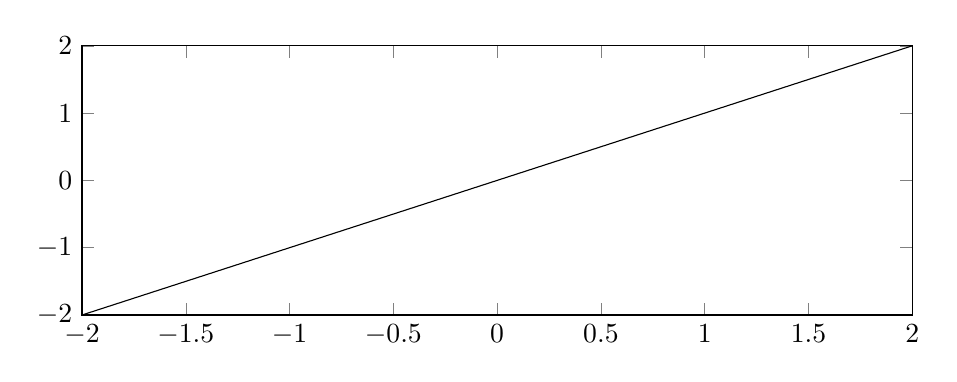
\begin{tikzpicture}
        \begin{axis}[
          width=\textwidth,
          height=5cm,
          xmin=-2,
          xmax=2,
          ymin=-2,
          ymax=2
        ]
          \addplot[black, domain=-2:2, samples=100] {x};
        \end{axis}
      \end{tikzpicture}
      \caption{Linear}
      \label{fig:plot1}
    \end{subfigure}
    \hfill
    \begin{subfigure}{0.3\textwidth}
        \centering
        \begin{tikzpicture}
          \begin{axis}[
            width=\textwidth,
            height=5cm,
            xmin=-2,
            xmax=2,
            ymin=-1.1,
            ymax=1.1,
            samples=100,
            xtick={-2,-1,0,1,2},
            ytick={-1,0,1},
            clip=false
          ]
            % Plot the sign function
            \addplot[black, thick, mark=none, domain=-2:0] {-1};
            \addplot[black, thick, mark=none, domain=0:2] {1};
            \draw (axis cs:0,-1) -- (axis cs:0,1);
          \end{axis}
        \end{tikzpicture}
        \caption{Sign Function}
        \label{fig:plot2}
      \end{subfigure}
    \hfill
    \begin{subfigure}{0.3\textwidth}
      \centering
      \begin{tikzpicture}
        \begin{axis}[
          width=\textwidth,
          height=5cm,
          xmin=-15,
          xmax=15,
          ymin=-1,
          ymax=1.1
        ]
          % Plot 3 data and settings
          \addplot[black, domain=-15:15, samples=100] {1/(1 + exp(-x))};
        \end{axis}
      \end{tikzpicture}
      \caption{Sigmoid}
      \label{fig:plot3}
    \end{subfigure}
  
    \medskip
  
    \begin{subfigure}{0.3\textwidth}
      \centering
      \begin{tikzpicture}
        \begin{axis}[
          width=\textwidth,
          height=5cm,
          xmin=-6.5,
          xmax=6.5,
          ymin=-1.1,
          ymax=1.1
        ]
          % Plot 4 data and settings
          \addplot[black, domain=-6.5:6.5, samples=100] {(exp(2*x)-1)/(exp(2*x)+1)};
        \end{axis}
      \end{tikzpicture}
      \caption{Tanh}
      \label{fig:plot4}
    \end{subfigure}
    \hfill
    \begin{subfigure}{0.3\textwidth}
      \centering
      \begin{tikzpicture}
        \begin{axis}[
            width=\textwidth,
            height=5cm,
            xmin=-2,
            xmax=2,
            ymin=-1.1,
            ymax=1.1
        ]
          % Plot 5 data and settings
          \addplot[black, domain=-2:2, samples=100] {max(x,0)};
        \end{axis}
      \end{tikzpicture}
      \caption{ReLU}
      \label{fig:plot5}
    \end{subfigure}
    \hfill
    \begin{subfigure}{0.3\textwidth}
      \centering
      \begin{tikzpicture}
        \begin{axis}[
            width=\textwidth,
            height=5cm,
            xmin=-2,
            xmax=2,
            ymin=-1.1,
            ymax=1.1
        ]
          % Plot 6 data and settings
          \addplot[black, domain=-2:2, samples=100] {max(min(x,1),-1)};
        \end{axis}
      \end{tikzpicture}
      \caption{Hard Tanh}
      \label{fig:plot6}
    \end{subfigure}
  
    \caption{Aktivierungsfunktionen}
    \label{fig:grid}
  \end{figure}
  
  TEXT FOLGT... 


\newpage
\subsubsection{Schichtenmodell}\label{subsec:neuronen:schichtenmodell}
  %\input{}
  TEXT FOLGT... 

\subsubsection{Loss-Function}

\newpage 
\subsection{Wie sind Neuronen miteinander verknüpft}\label{subsec:neuronen:verknuepfung_neuronen}  
%\input{}
Hier sollen die Weights erklärt werden

\subsubsection{Weights}\label{Weights}
  %\input{}
  TEXT FOLGT... 

\subsection{Fehler / Backpropagation Einführung}\label{subsec:neuronen:fehler_backpropagation}
Nur eine sehr knappe Einführung, da eigenes Kapitel für dieses Thema reserviert

